% Figura Anexo II: una mejora de la productividad en el mercado de trabajo: sin oferta elástica no hay ciclo
\documentclass[tikz,border=3pt]{standalone}
\usepackage[T1]{fontenc}
\usepackage[utf8]{inputenc}
\usepackage{amsmath}
\usetikzlibrary{arrows.meta,calc,positioning}
\begin{document}
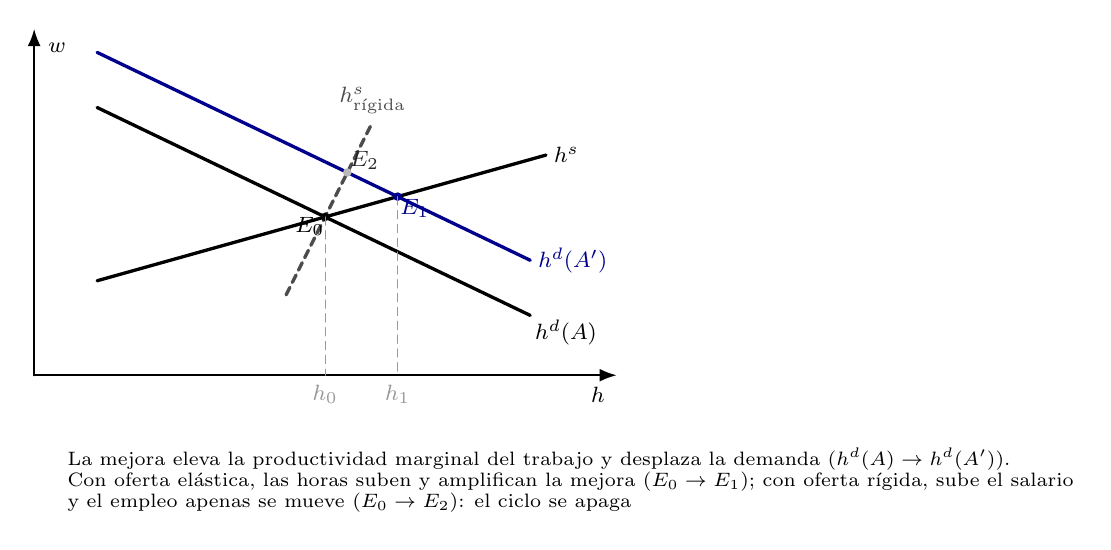
\begin{tikzpicture}[>={Latex[length=2.2mm]}, line cap=round, font=\footnotesize,
  eje/.style={->, thick},
  curva/.style={very thick},
  nueva/.style={very thick, blue!55!black},
  guia/.style={densely dashed, gray!80},
  pto/.style={circle, fill=black, inner sep=1.1pt}]
  \draw[eje] (0,0) -- (7.4,0) node[below left=1pt]{$h$};
  \draw[eje] (0,0) -- (0,4.4) node[below right=2pt]{$w$};
  % demanda de trabajo: w = 3.784 - 0.48 h
  \draw[curva] (0.8,3.4) -- (6.3,0.76) node[below right=-3pt]{$h^{d}(A)$};
  \draw[nueva] (0.8,4.1) -- (6.3,1.46) node[right=-1pt]{$h^{d}(A')$};
  % oferta elastica: w = 0.976 + 0.28 h
  \draw[curva] (0.8,1.2) -- (6.5,2.796) node[right=-1pt]{$h^{s}$};
  % oferta poco elastica por E0
  \draw[curva, gray!60!black, densely dashed] (3.2,1.021) -- (4.3,3.221) node[above=-1pt]{$h^{s}_{\text{rígida}}$};
  \node[pto] (E0) at (3.695,2.011) {};
  \node[below left=-3pt of E0, inner sep=1pt] {$E_0$};
  \node[pto, fill=blue!55!black] (E1) at (4.616,2.268) {};
  \node[below right=-2pt of E1, inner sep=1pt, blue!55!black] {$E_1$};
  \node[pto, fill=gray!55] (E2) at (3.977,2.575) {};
  \node[above right=-2pt of E2, inner sep=1pt, gray!30!black] {$E_2$};
  \draw[guia] (3.695,2.011) -- (3.695,0) node[below]{$h_0$};
  \draw[guia] (4.616,2.268) -- (4.616,0) node[below]{$h_1$};
  \node[align=left, anchor=north west] at (0.3,-0.8) {\scriptsize La mejora eleva la productividad marginal del trabajo y desplaza la demanda ($h^{d}(A)\to h^{d}(A')$).\\[-2pt]\scriptsize Con oferta elástica, las horas suben y amplifican la mejora ($E_0\to E_1$); con oferta rígida, sube el salario\\[-2pt]\scriptsize y el empleo apenas se mueve ($E_0\to E_2$): el ciclo se apaga};
\end{tikzpicture}
\end{document}
